
\subsection{SHM relation}
The SHM relation for all the galaxies, as well as only the central galaxies, with $M_{*} > 10^8 M_{\odot}$ from TNG is plotted in figure \ref{shmr_res}, along with the best fits from \cite{Moster2012}, \cite{Behroozi2013} and \cite{Zanisi2019}.
When calculating the SHM relation using all the galaxies, the median values are pushed towards lower halo masses compared to only central galaxies. As mentioned earlier, the central galaxies are less affected by environmental conditions, and so they better reflect the ``isolated galaxy evolution''. Compared to the data, the central galaxy SHM relation falls right in between the fits from Moster et al. and Behroozi et al. for lower mass galaxies. However, the steepness of theslope is closer to that of Zainsi et al. Above the characteristic halo mass of $\approx 10^{11.6} M_{\odot}$, the TNG SHM relation deviates significantly from the abundance matching fit by having a much steeper slope. This indicates a value for $\gamma$ in equation \ref{eq_behroozi} closer to unity. The more recent, centrals only, results from Zanisi et al. agrees better with the high mass slope than the other two, but the difference is still significant. This is expected, and other works show similar results (check)


\begin{figure}
    \centering
    \makebox[\textwidth][c]{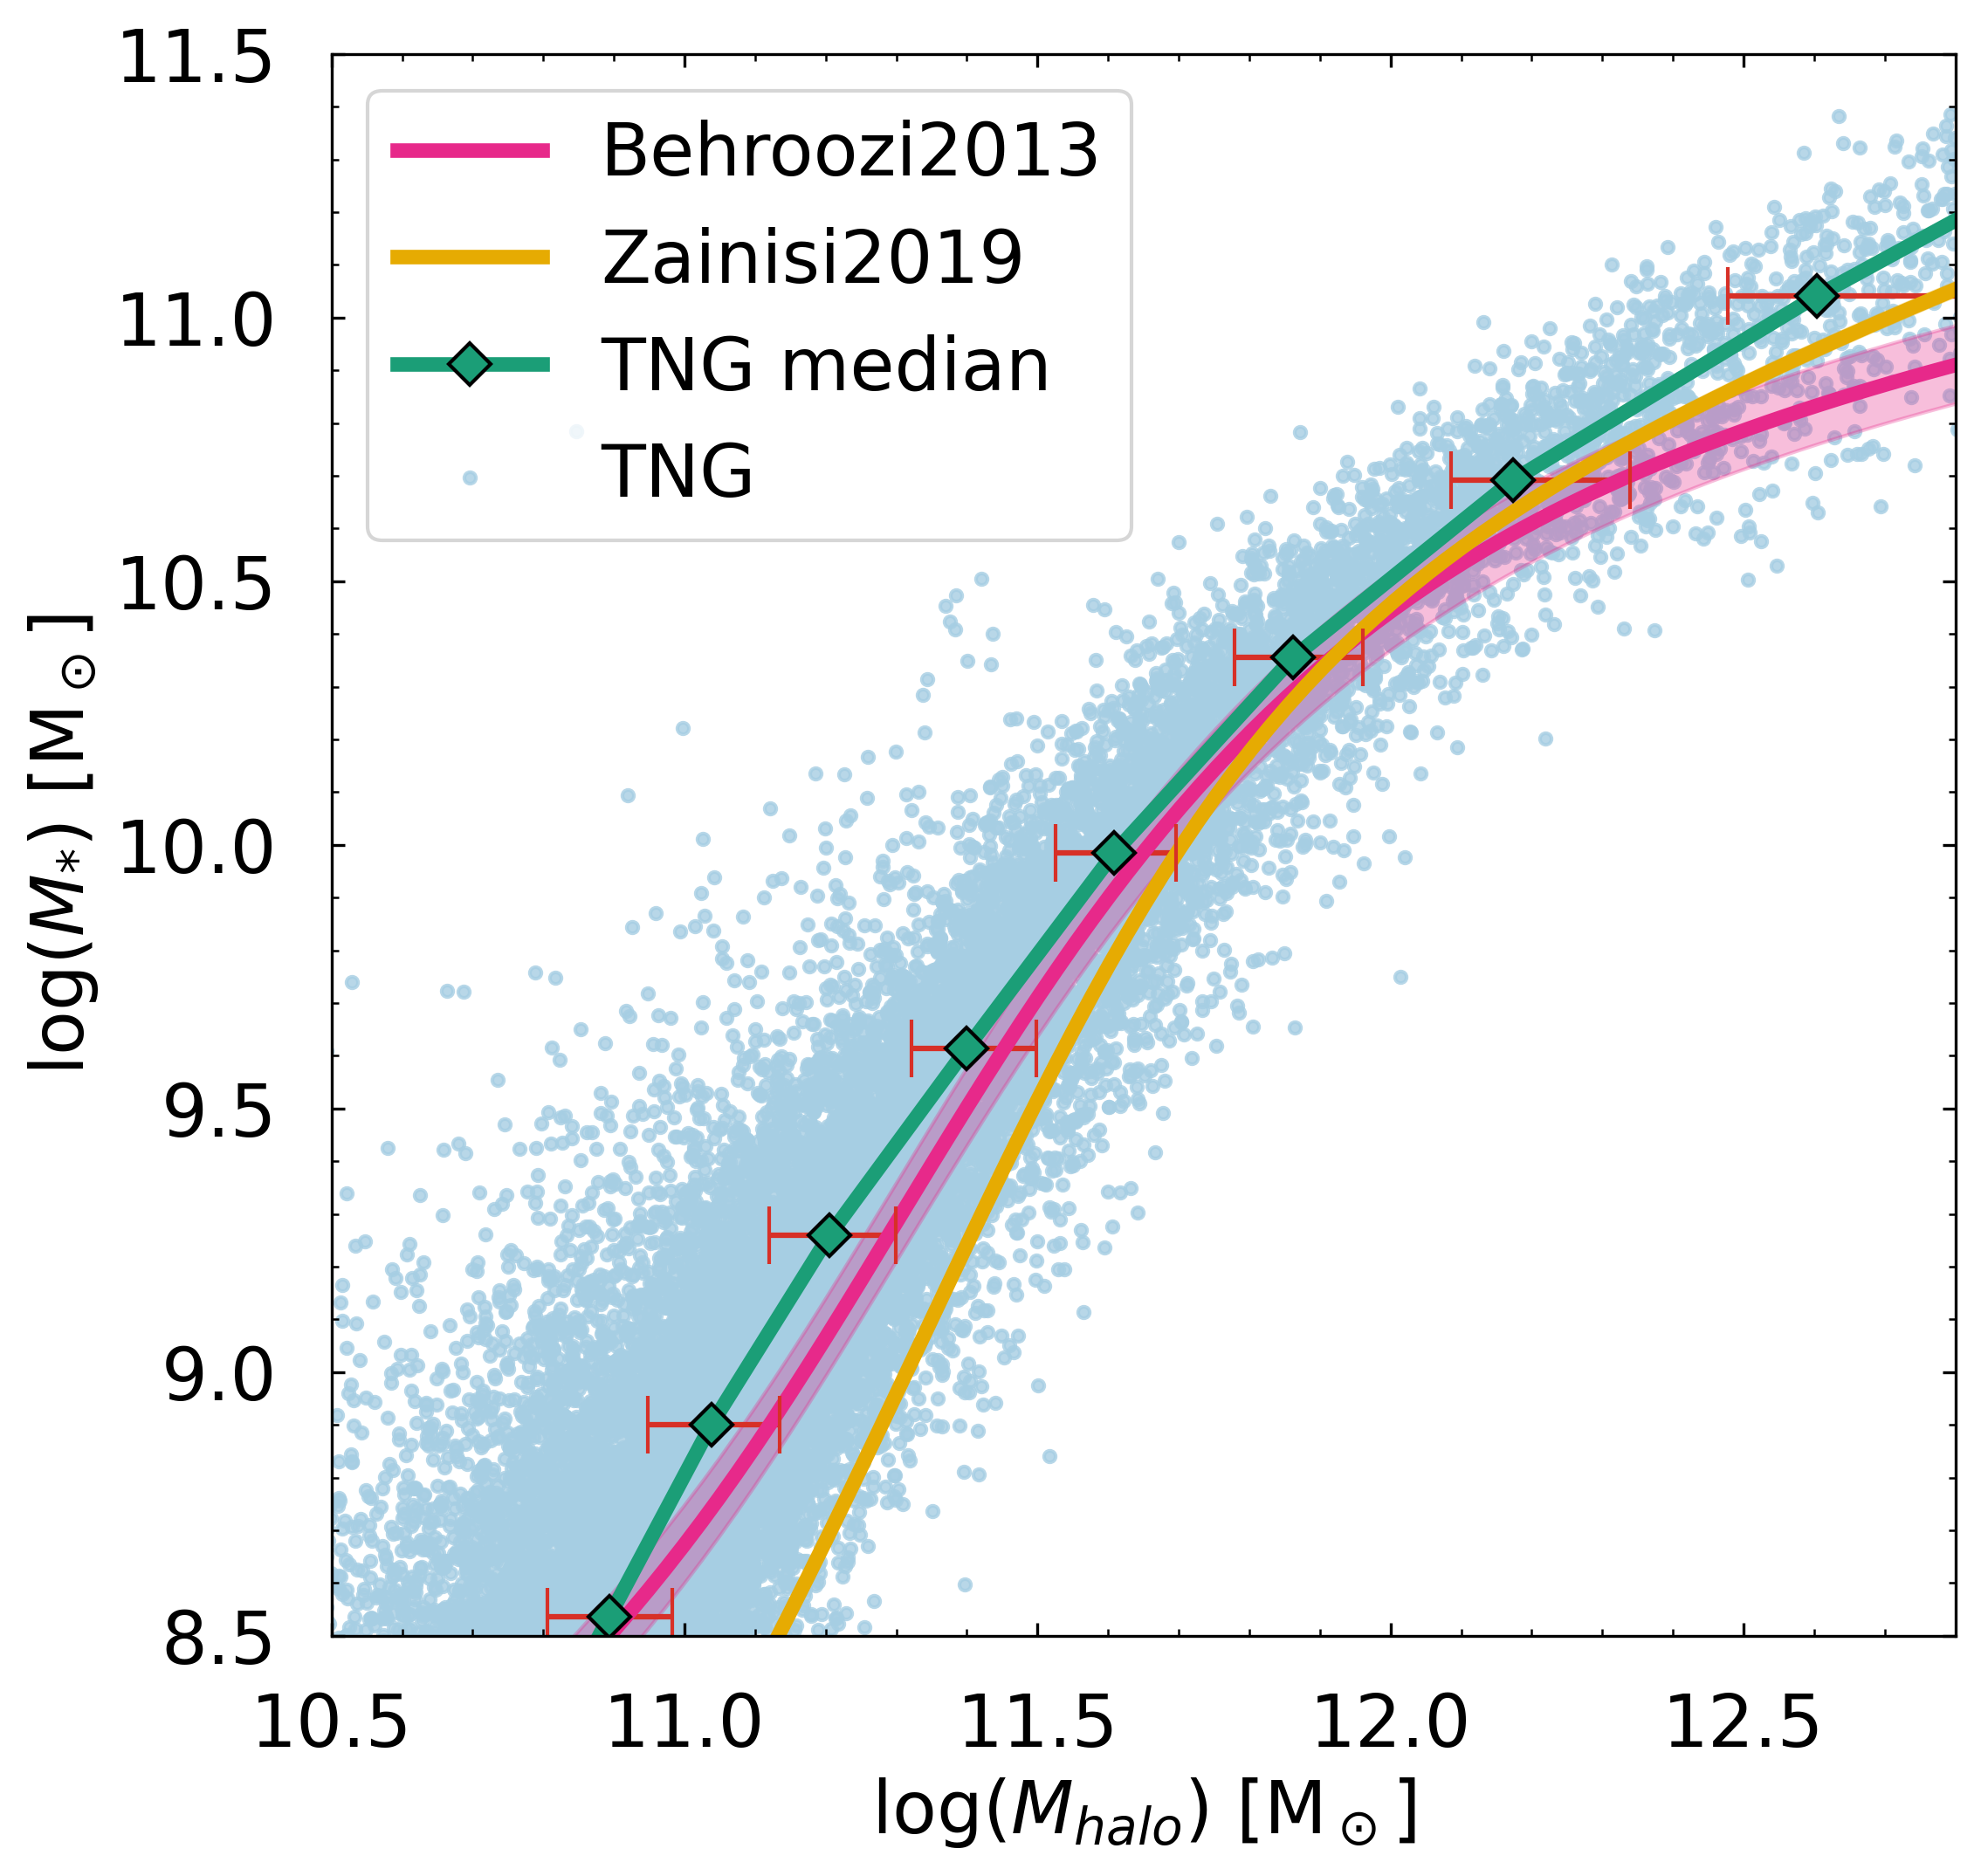
\includegraphics[width=0.9\paperwidth]{images/results_shmr.png}}
    \caption{The SHM relation of the TNG simulation for all galaxies above stellar mass $10^8 M_{\odot}$. The best fit from abundance matching from three different papers (\cite{Moster2012}, \cite{Behroozi2013} and \cite{Zanisi2019}) are also shown.} 
    \label{shmr_res}
\end{figure}


\subsection{TFR}
The TFR for the late type galaxies in TNG is shown in Figure \ref{tfr_res} along with the best fit for the SAMI data found in \cite{Bloom2017}. The slope of the TNG TFR seems to be slightly steeper than for \cite{Bloom2017}. Rotational velocities for TNG are chosen as the maximum velocity in the velocity curve, while Bloom et al. use the velocity at $r = 2.2 r_e$. This could lead to the velocity measurements of the smaller galaxies being systematically lower for Bloom et al. compared to TNG. A better comparison would be to choose the same definition for the rotational velocity for both data sets. Also, it might be interesting to investiagte the Baryonic Tuller-Fisher relation by adding the HI-mass and velocity measurements to the stellar measurements.

\begin{figure}
    \centering
    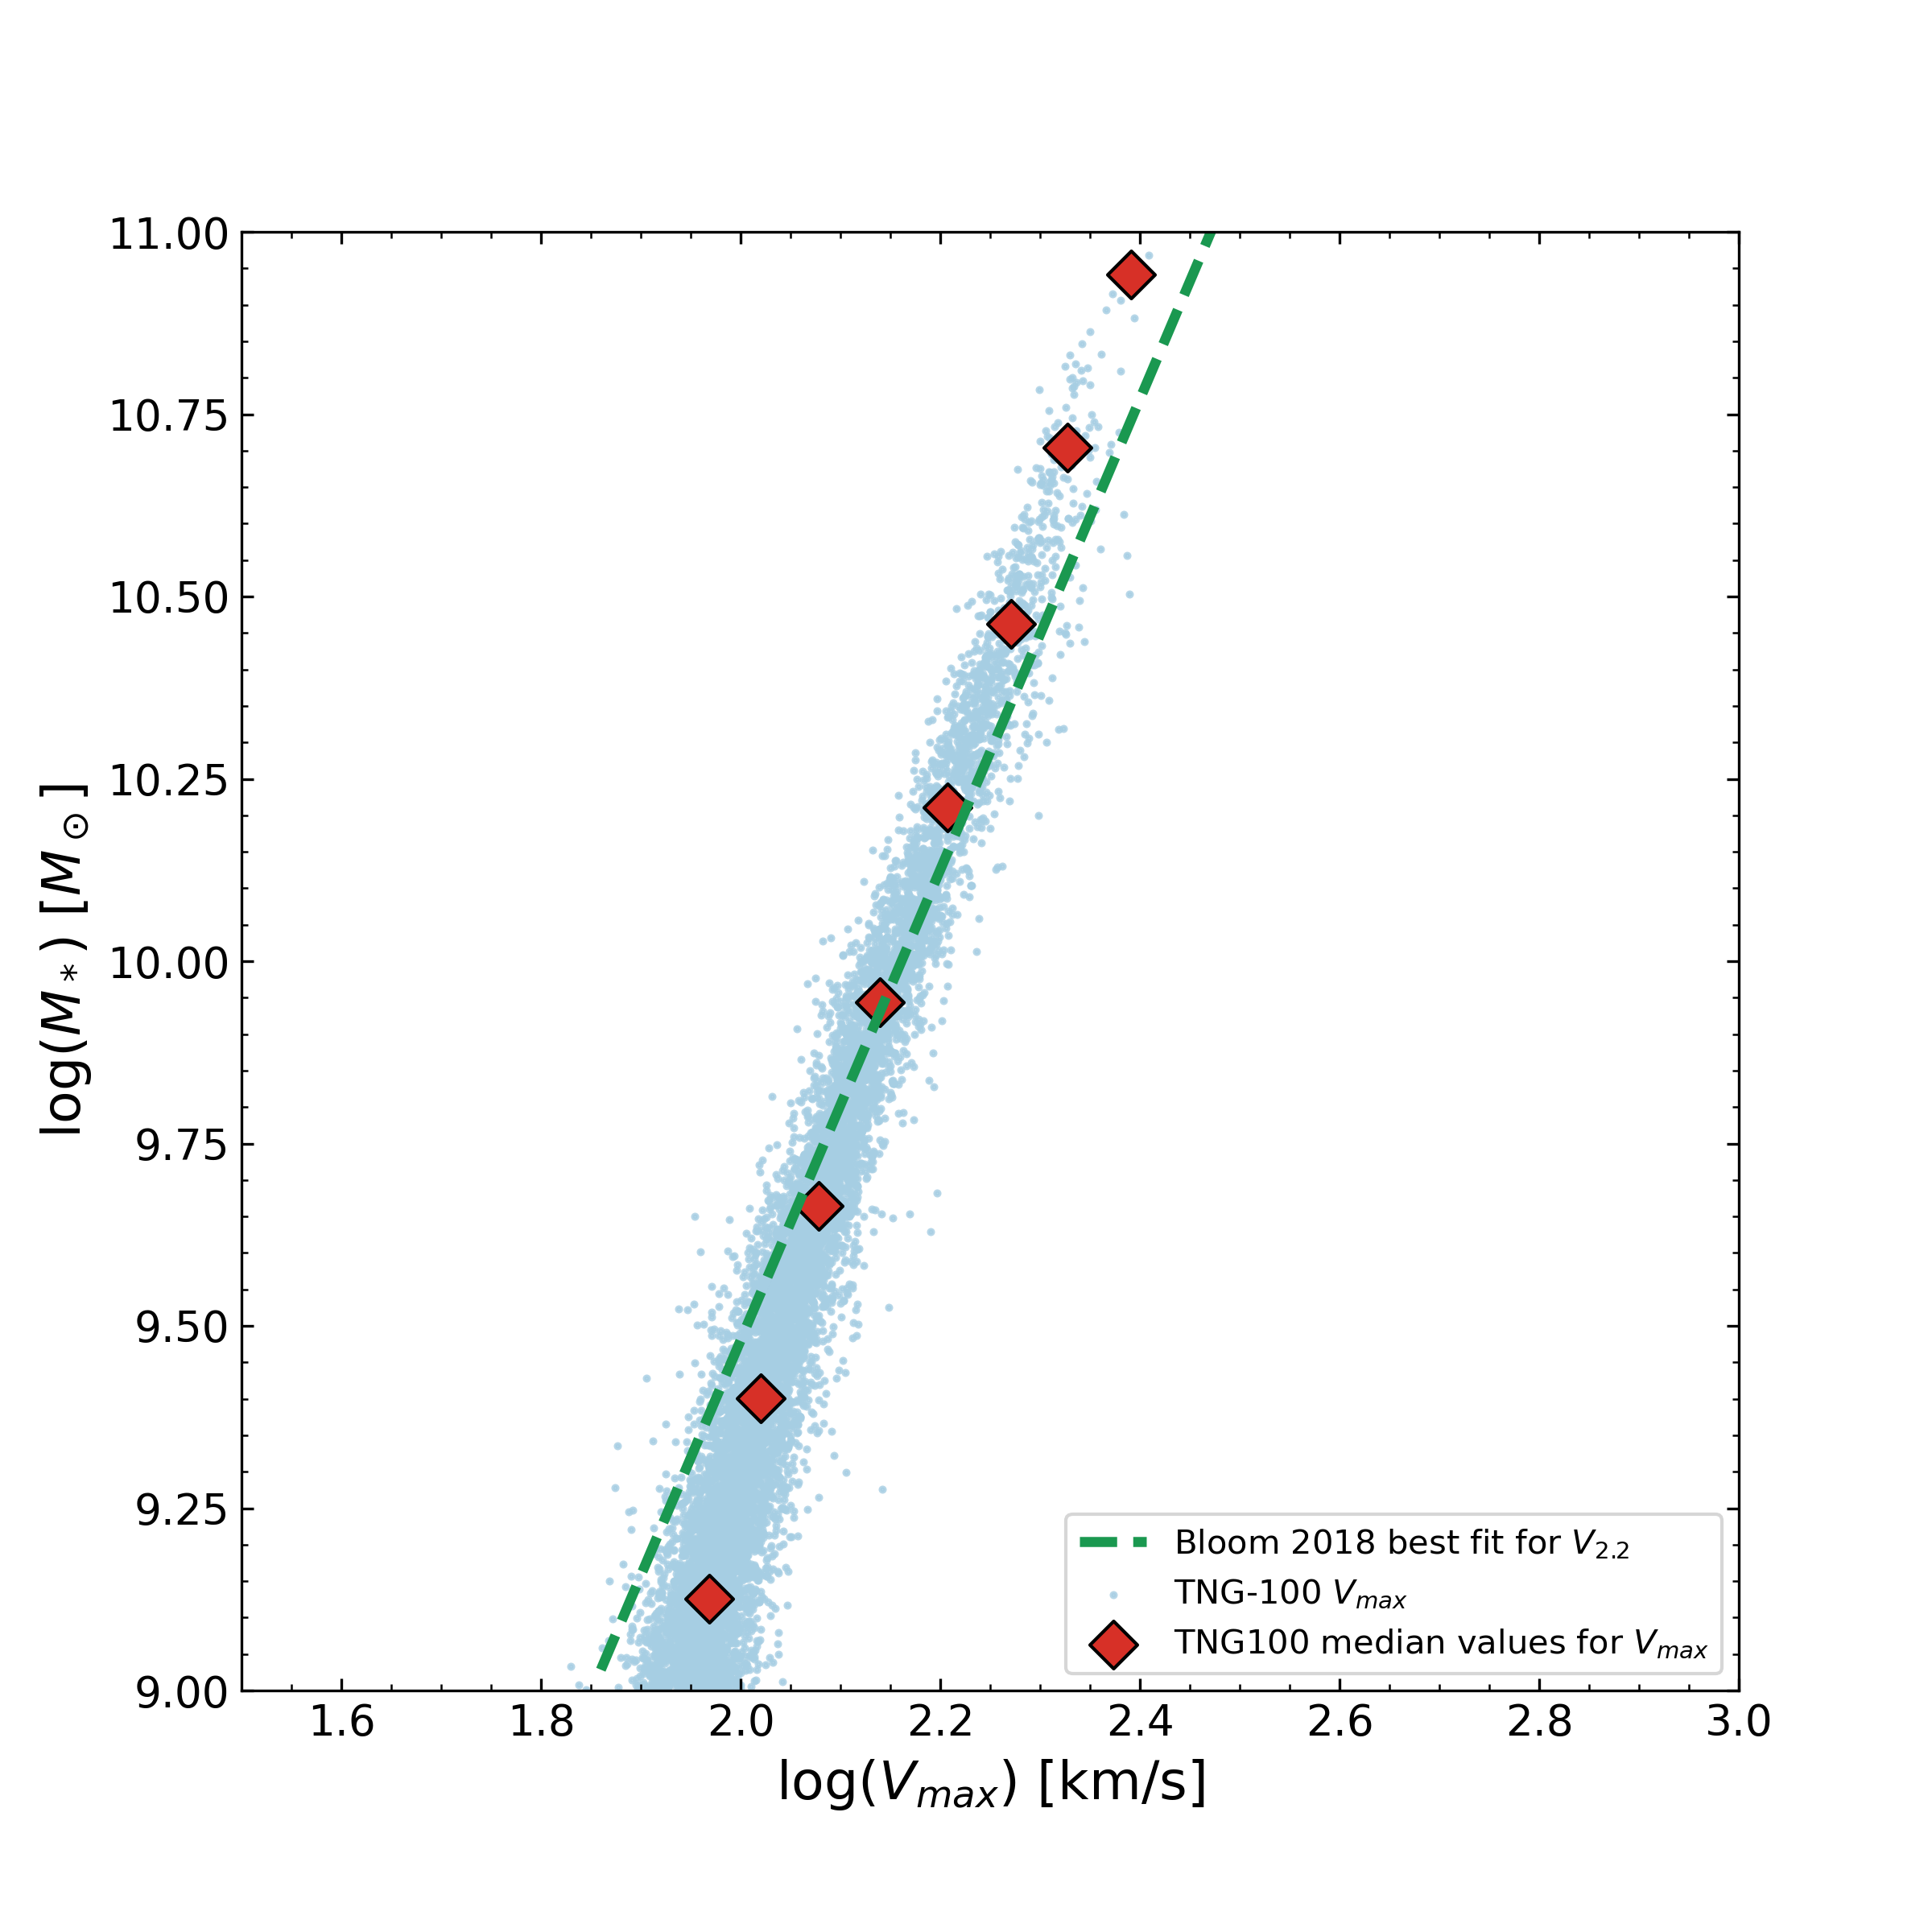
\includegraphics[width=0.9\textwidth]{images/results_tully_fisher.png}
    \caption{}
    \label{tfr_res}
\end{figure}

\subsection{FJ relation and the FP}

The velocity dispersion as function of stellar mass can be seen in Figure \ref{FJ_res}. The trend for the TNG-100 data is a clear power law as expected from the FJ relation. Compared to the observational data, the simulation data shows lower $\sigma$ values, by about 0.1-0.2 dex. This could be explained by the fact that the $\sigma$ in the TNG galaxies is averaged across all particles, across the whole size of the subhalo. In general, gas has a lower $\sigma$ than stars and dark matter, so this could push the total $\sigma$ down. However, in early-type galaxies there is little gas so the impact would be expected to be small. The fact that $\sigma$ is found by averaging across the entire subhalo would include particles further out than for the SAMI data in which the velocity dispersion is averaged inside the effective radius ($\sigma_{e}$) is used. Other studies have also found that simulations tend to get lower values for $\sigma$ \parencite{Sande2018}, so this might also just be a limitation of the simulations.

The other relations in the fundamental plane are shown in Figures \ref{FP_res1} and \ref{FP_res1}. The mass-radius relation for TNG is in excellent agreement with SAMI for larger galaxies. For galaxies with $M_*<10^9 M_{\odot}$, there are so few data points for SAMI that the comparison is not really meaningful. 

The $\sigma$-radius relation is also affected by the systematically lower $\sigma$ values for TNG. 

\begin{figure}
    \centering
    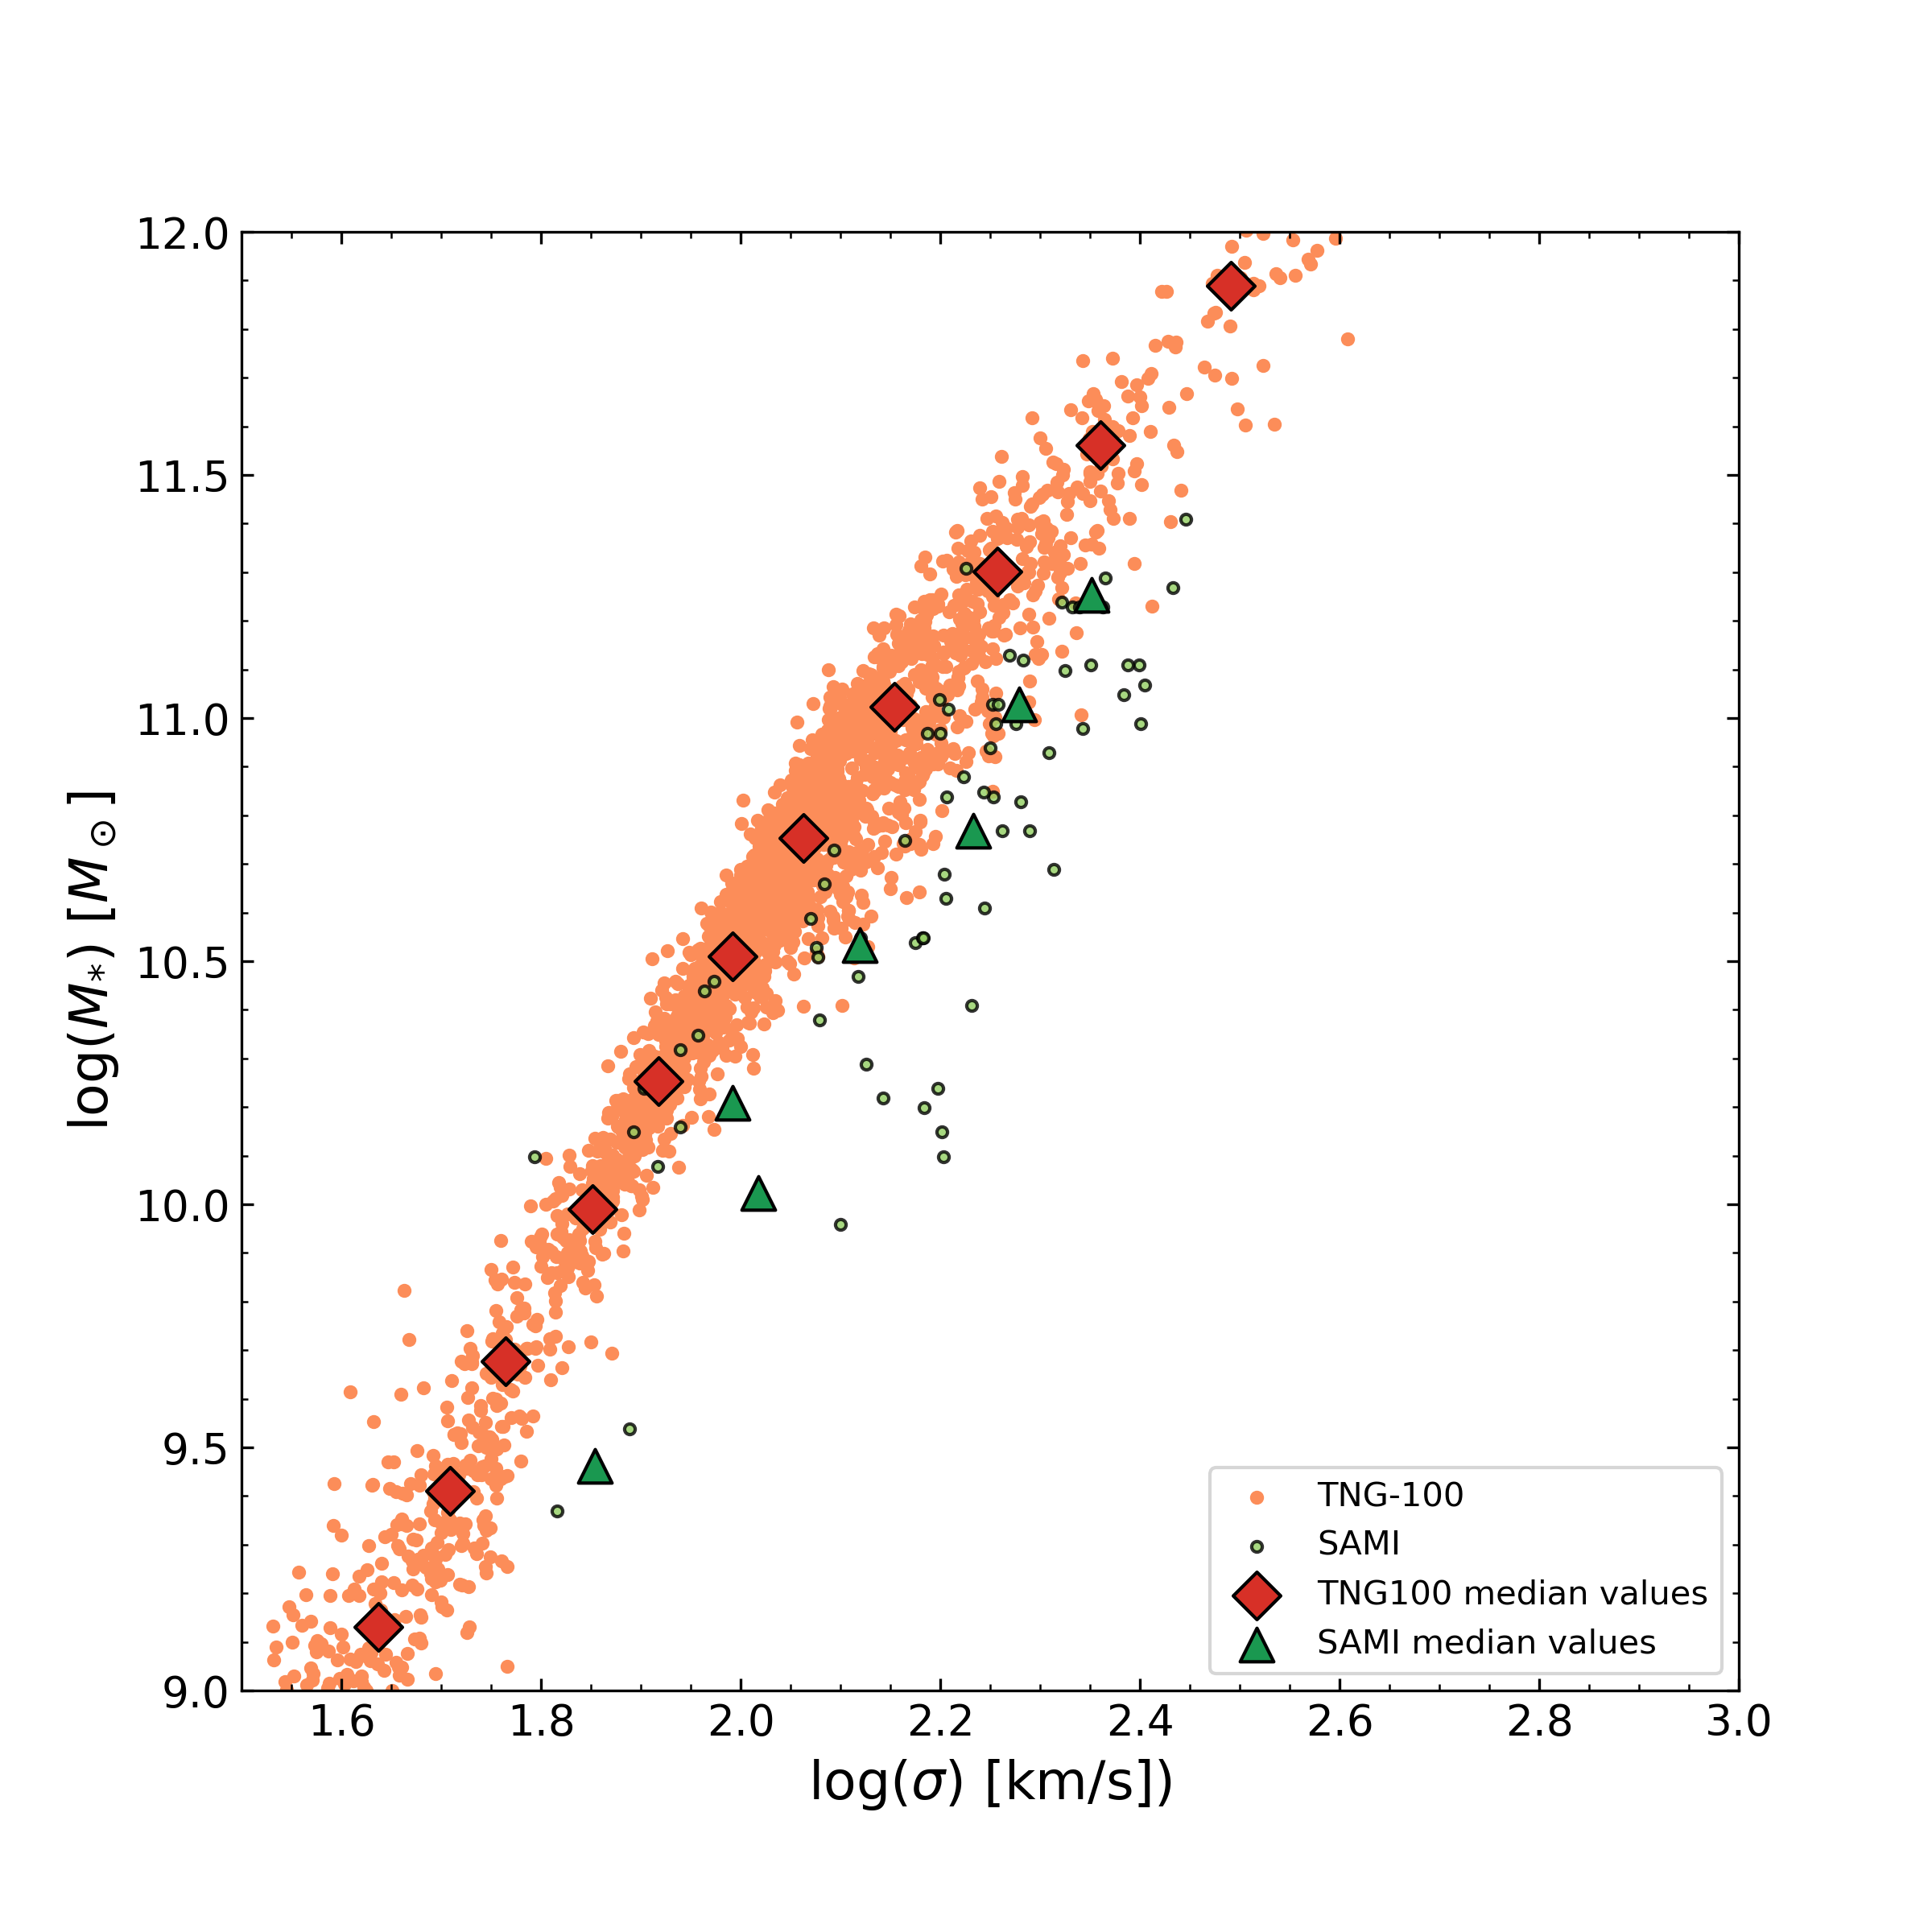
\includegraphics[width=\textwidth]{images/results_faber_jackson.png}
    \caption{Early type galaxies for both TNG and SAMI.}
    \label{FJ_res}
\end{figure}

\begin{figure}
    \centering
    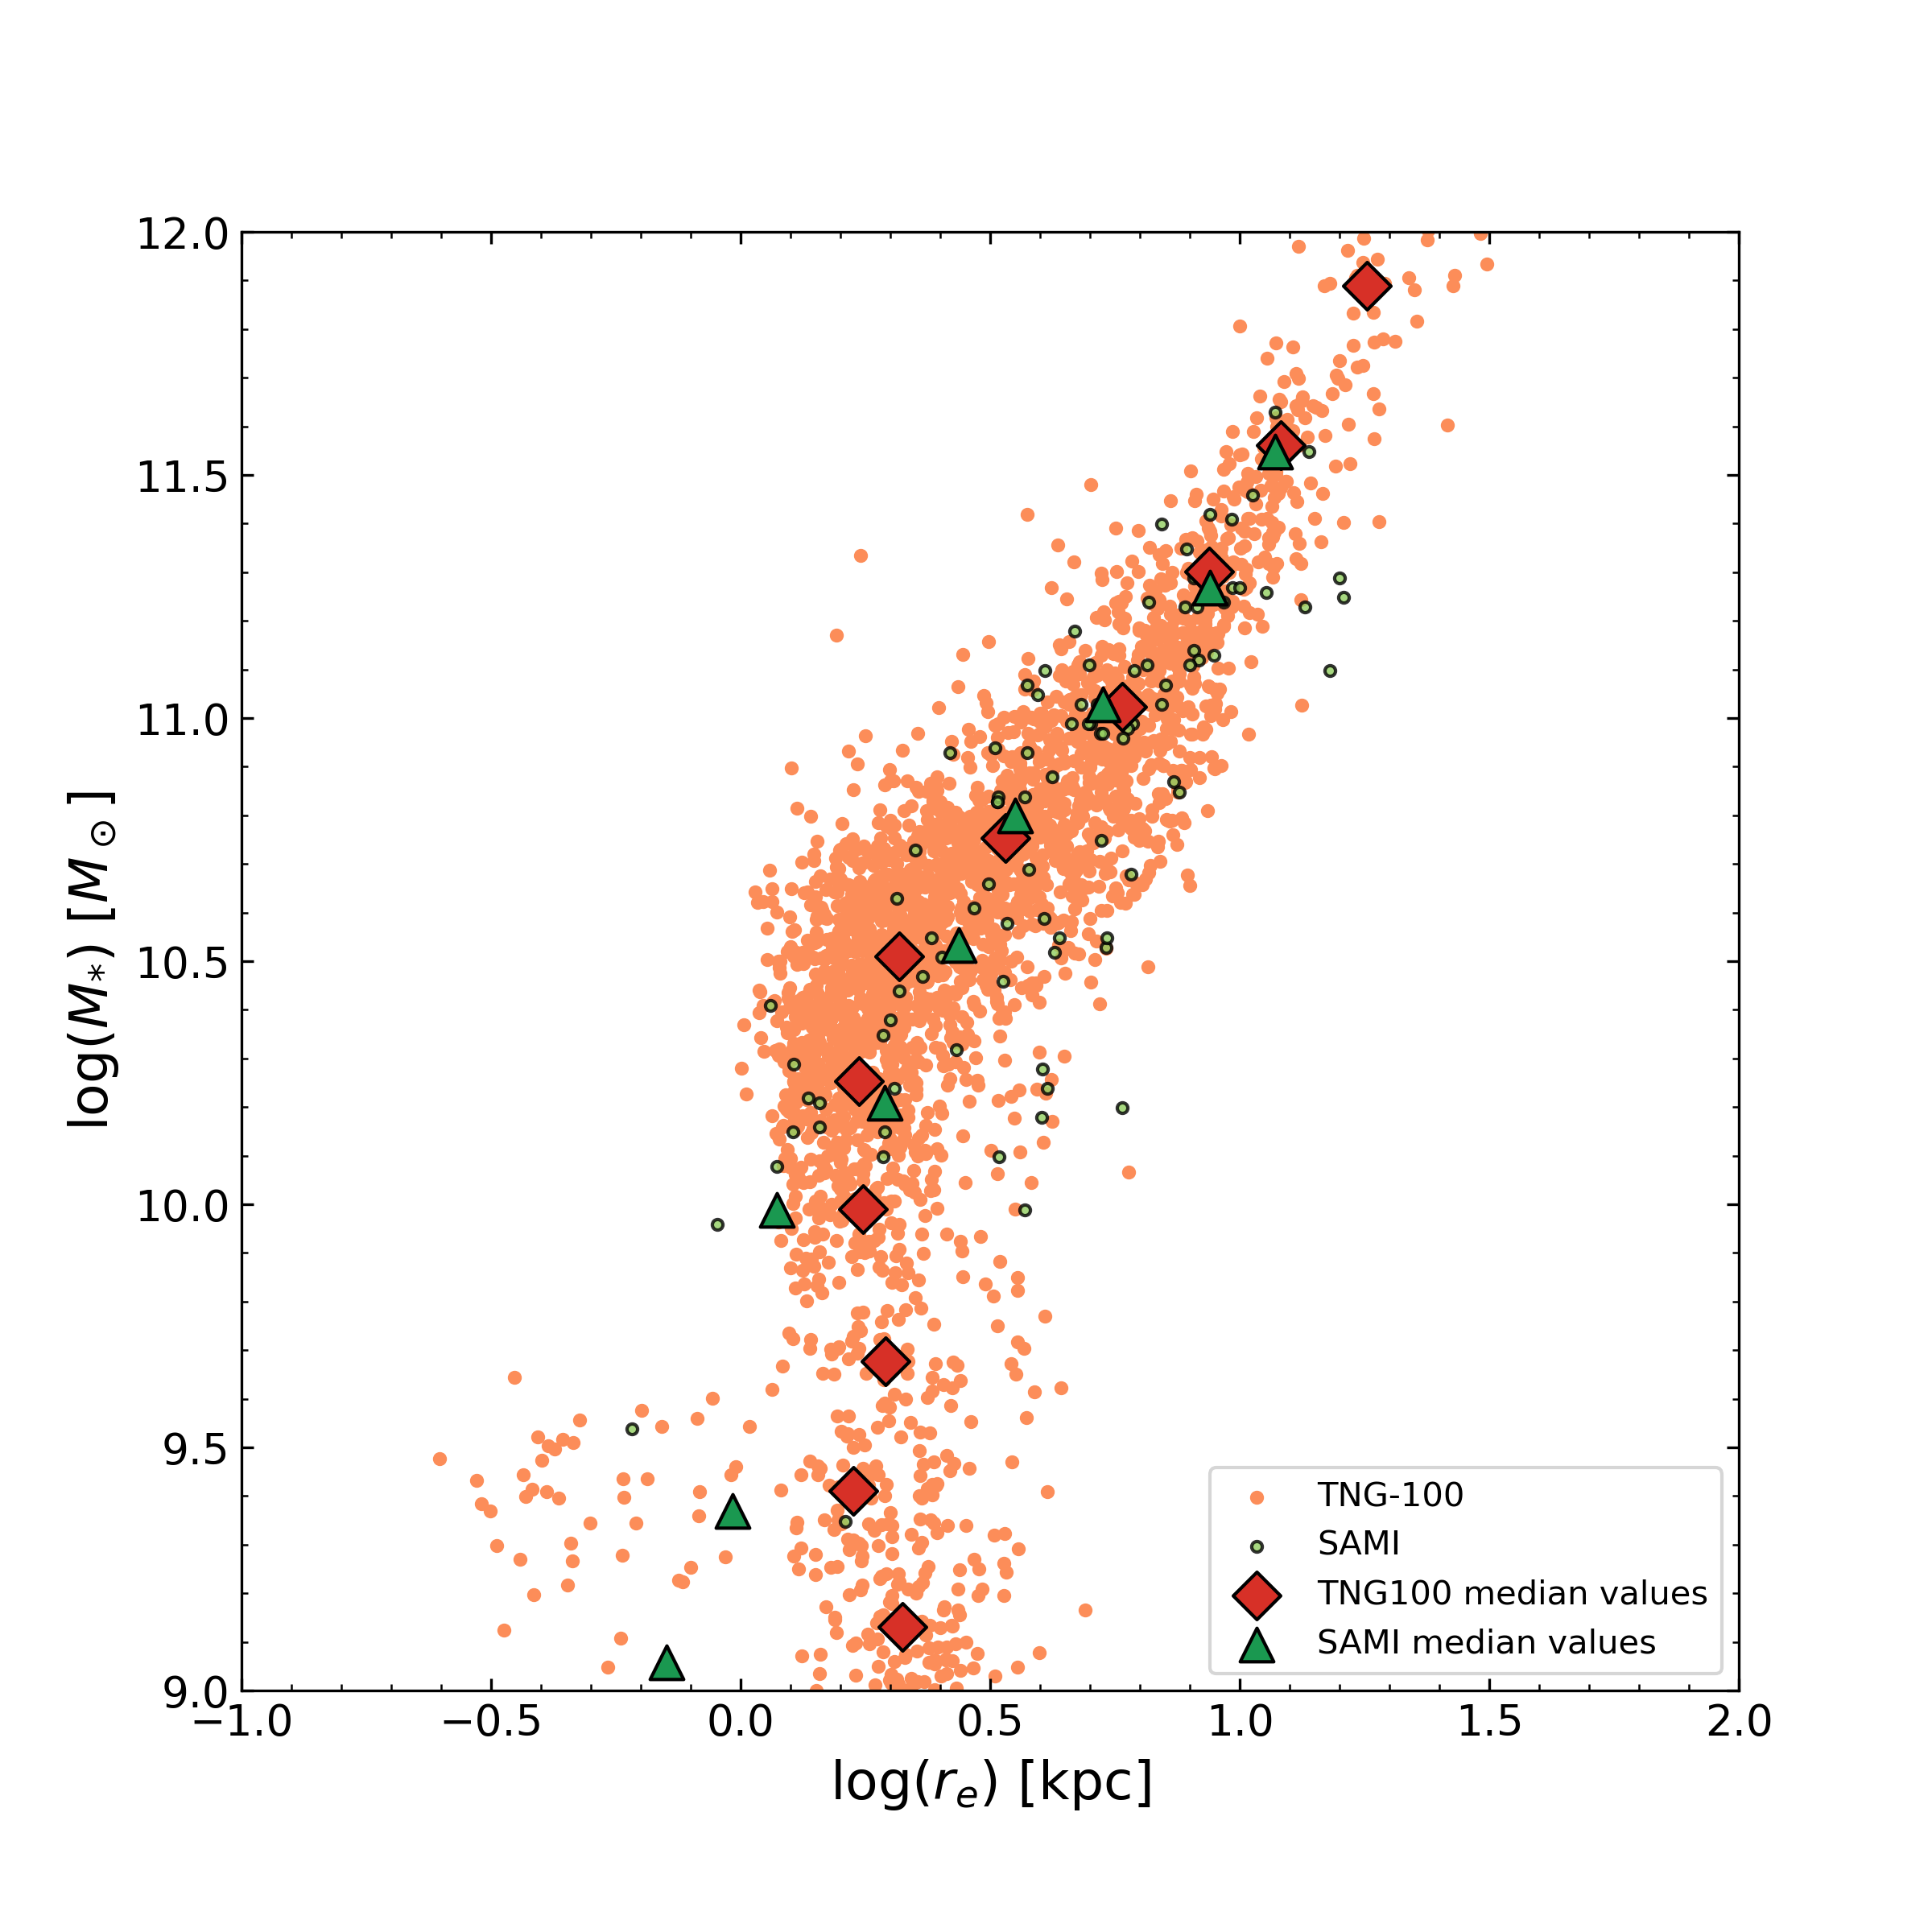
\includegraphics[width=\textwidth]{images/results_mass_radius_FP.png}
    \caption{Early type galaxies for both TNG and SAMI.}
    \label{FP_res1}
\end{figure}

\begin{figure}
    \centering
    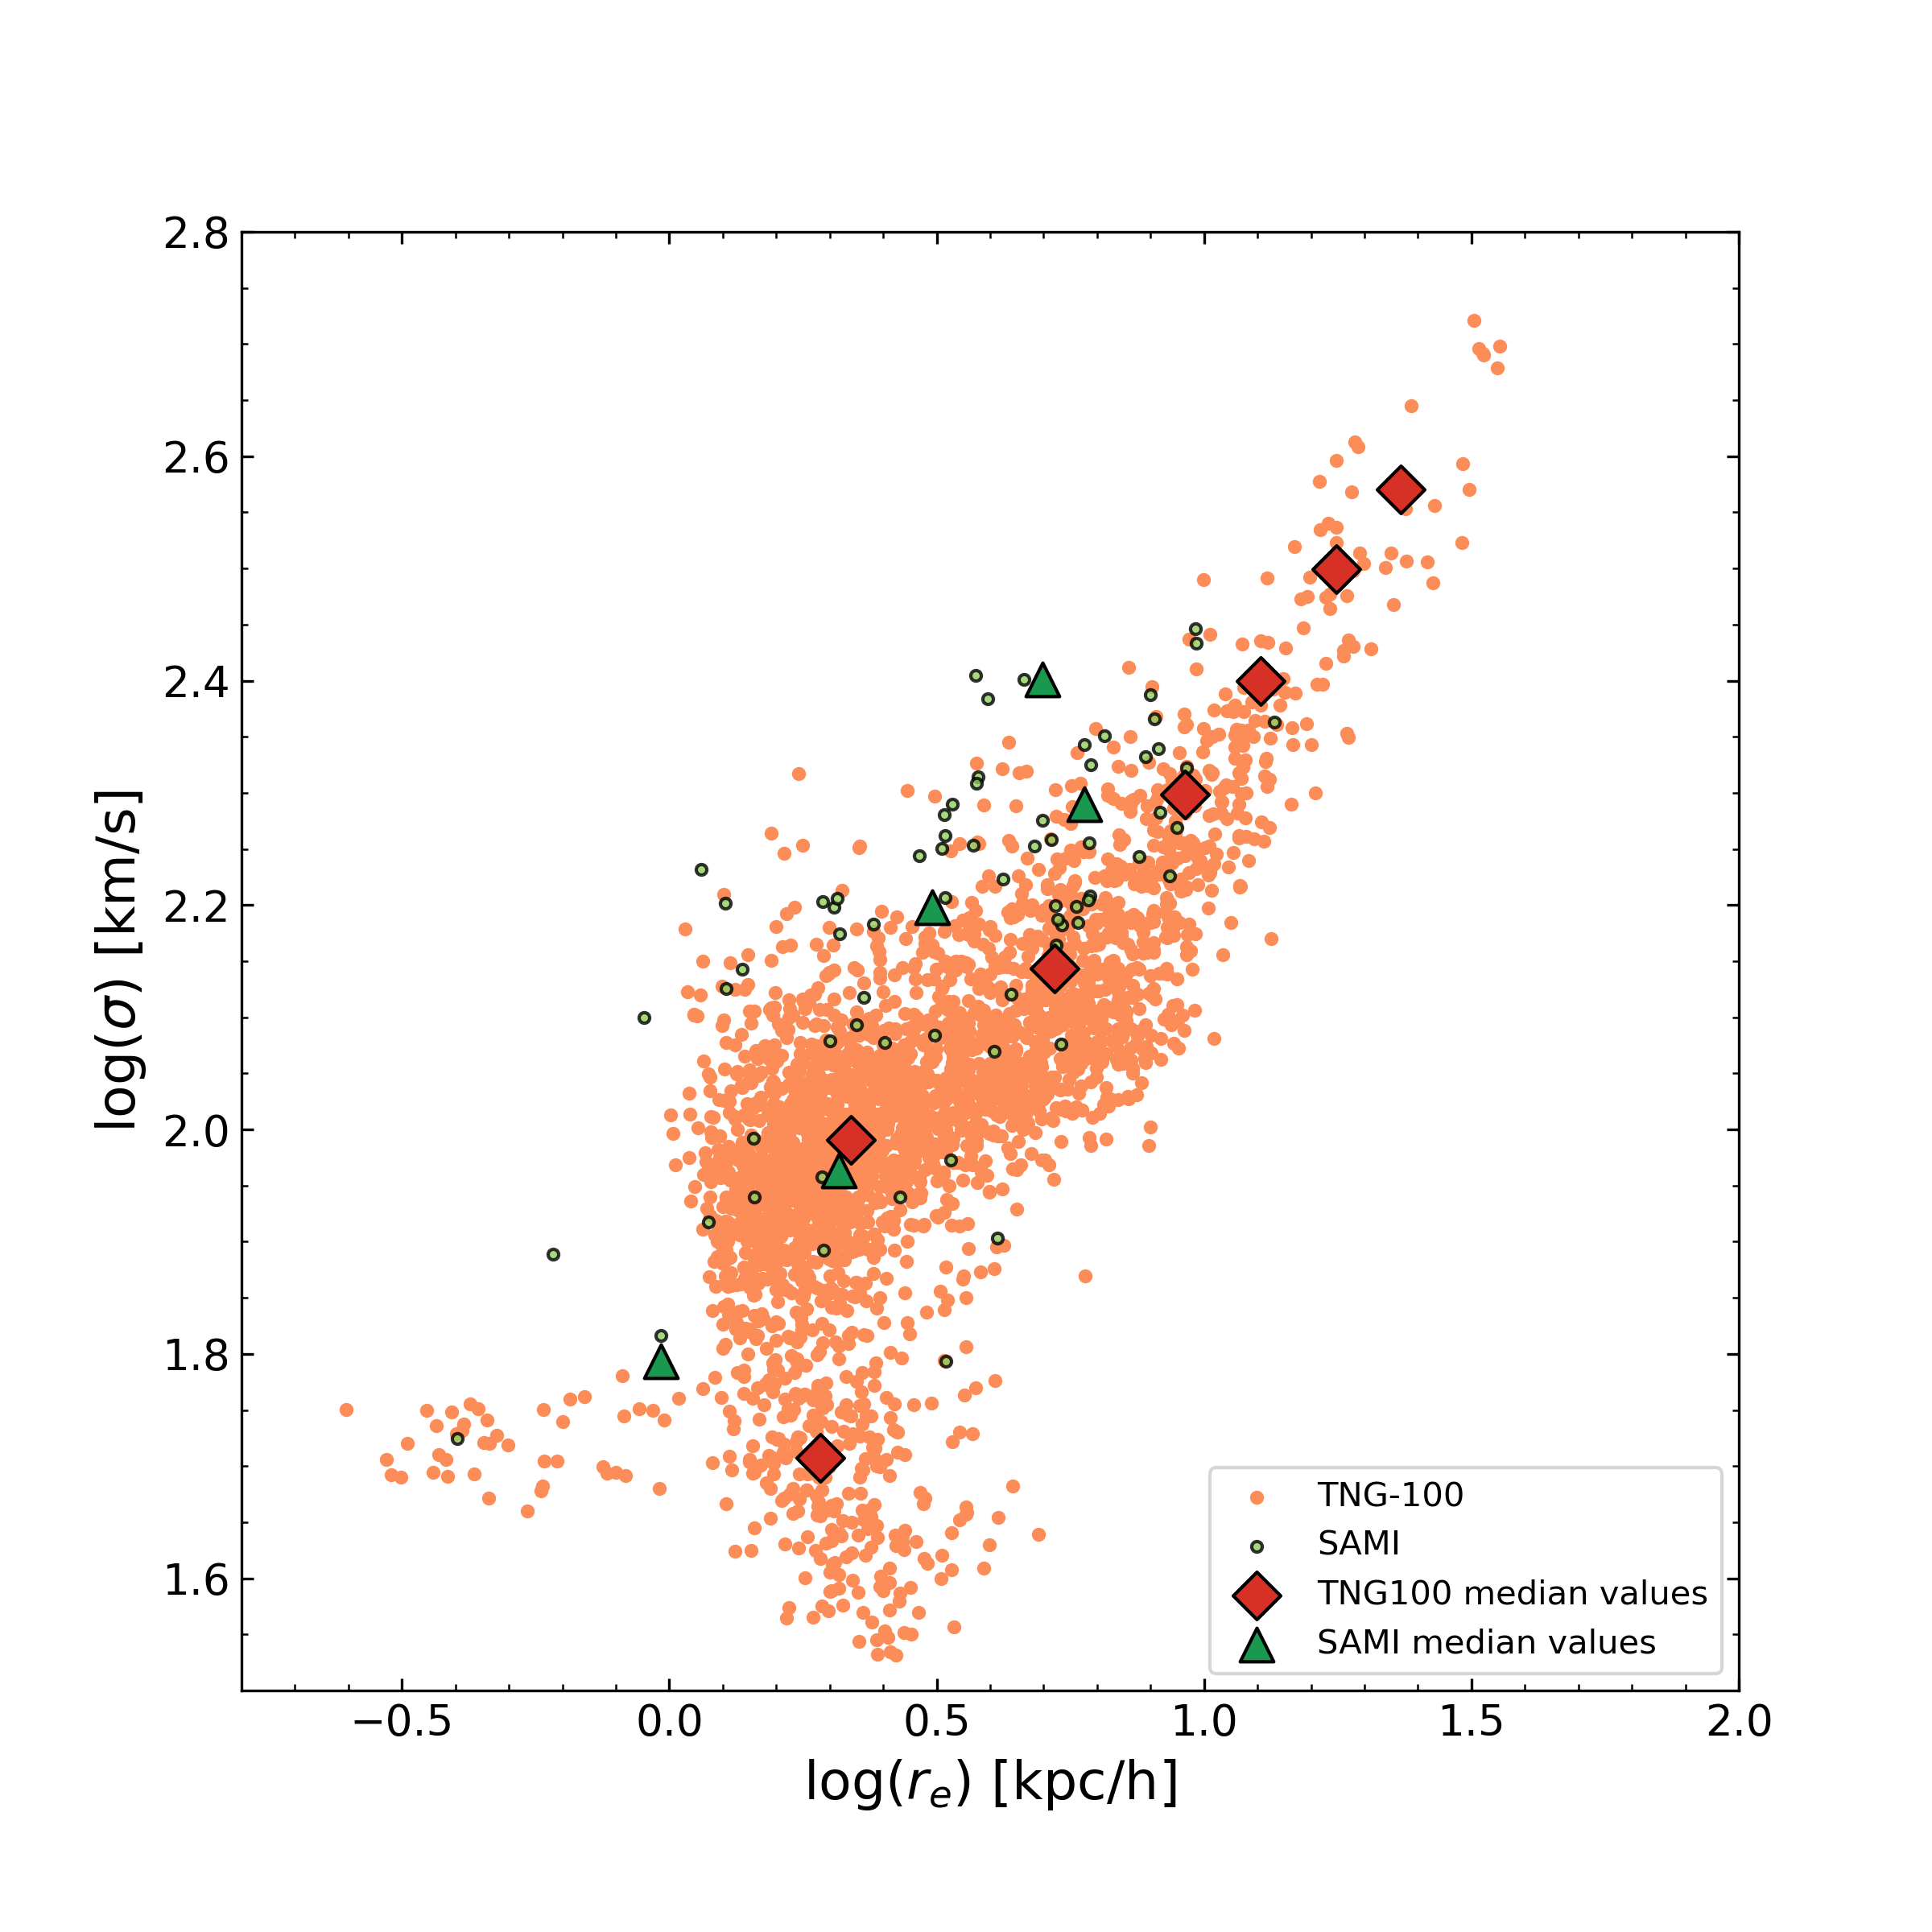
\includegraphics[width=\textwidth]{images/results_sigma_radius_FP.png}
    \caption{Early type galaxies for both TNG and SAMI.}
    \label{FP_res2}
\end{figure}

\subsection{Color bimodality}
The color-mass diagrams for different filters are shown in Figure \ref{color_magnitude_res}. There is a distinct serperation between early and late type galaxies, as expected. The distinction is clear in all bandfilters. 

Figure \ref{pdf_color_res1} shows the probability density function (PDF) for TNG100 early and late type galaxies for different filters. The separation into two main density peaks is apparent in all filters. In Figure \ref{pdf_color_res2} the PDF for the TNG100 (g-i) band and the SAMI (g-i) band are shown. The peaks coincide well for the two data sets, although the distribution in galaxies is different. This is likely because TNG has a larger amount of smaller, late-type blue galaxies, which are much more difficult to observe than larger and generally redder galaxies. A mass weighted PDF might give a more fair comparison.

\begin{figure}
    \centering
    \makebox[\textwidth][c]{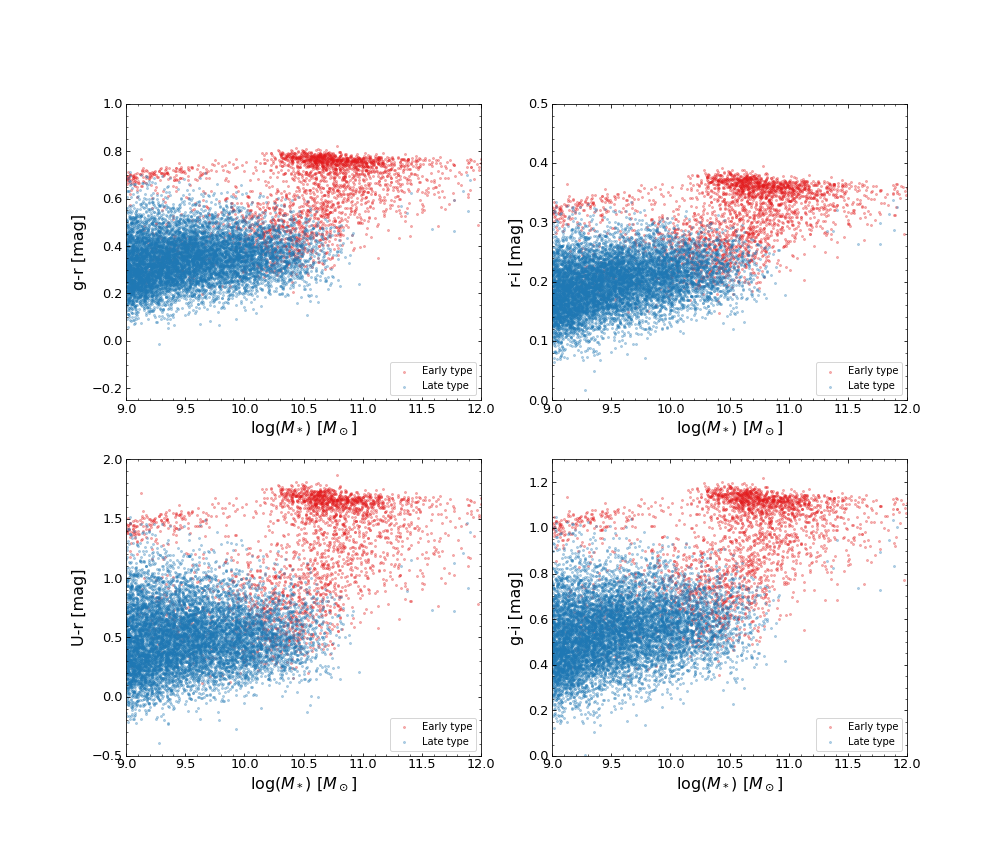
\includegraphics[width=0.9\paperwidth]{images/results_color_magnitude.png}}
    \caption{}
    \label{color_magnitude_res}
\end{figure}

\begin{figure}
    \centering
    \makebox[\textwidth][c]{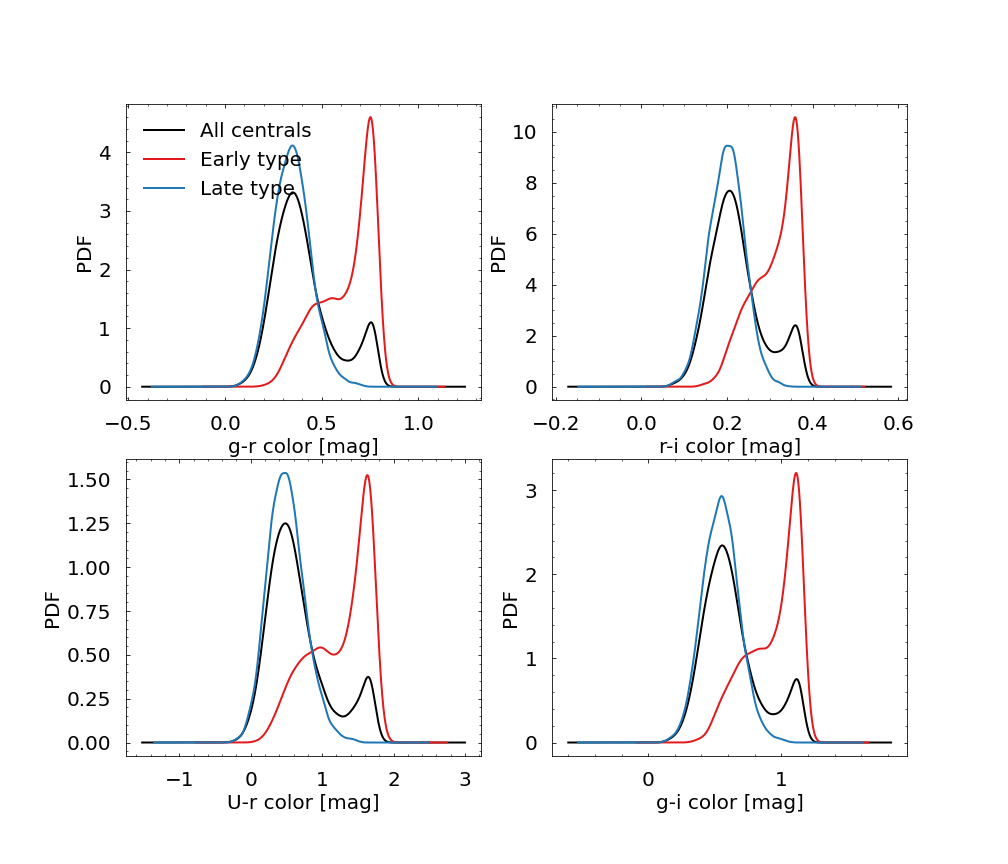
\includegraphics[width=0.9\paperwidth]{images/results_pdf_different_bands.png}}
    \caption{}
    \label{pdf_color_res1}
\end{figure}

\begin{figure}
    \centering
    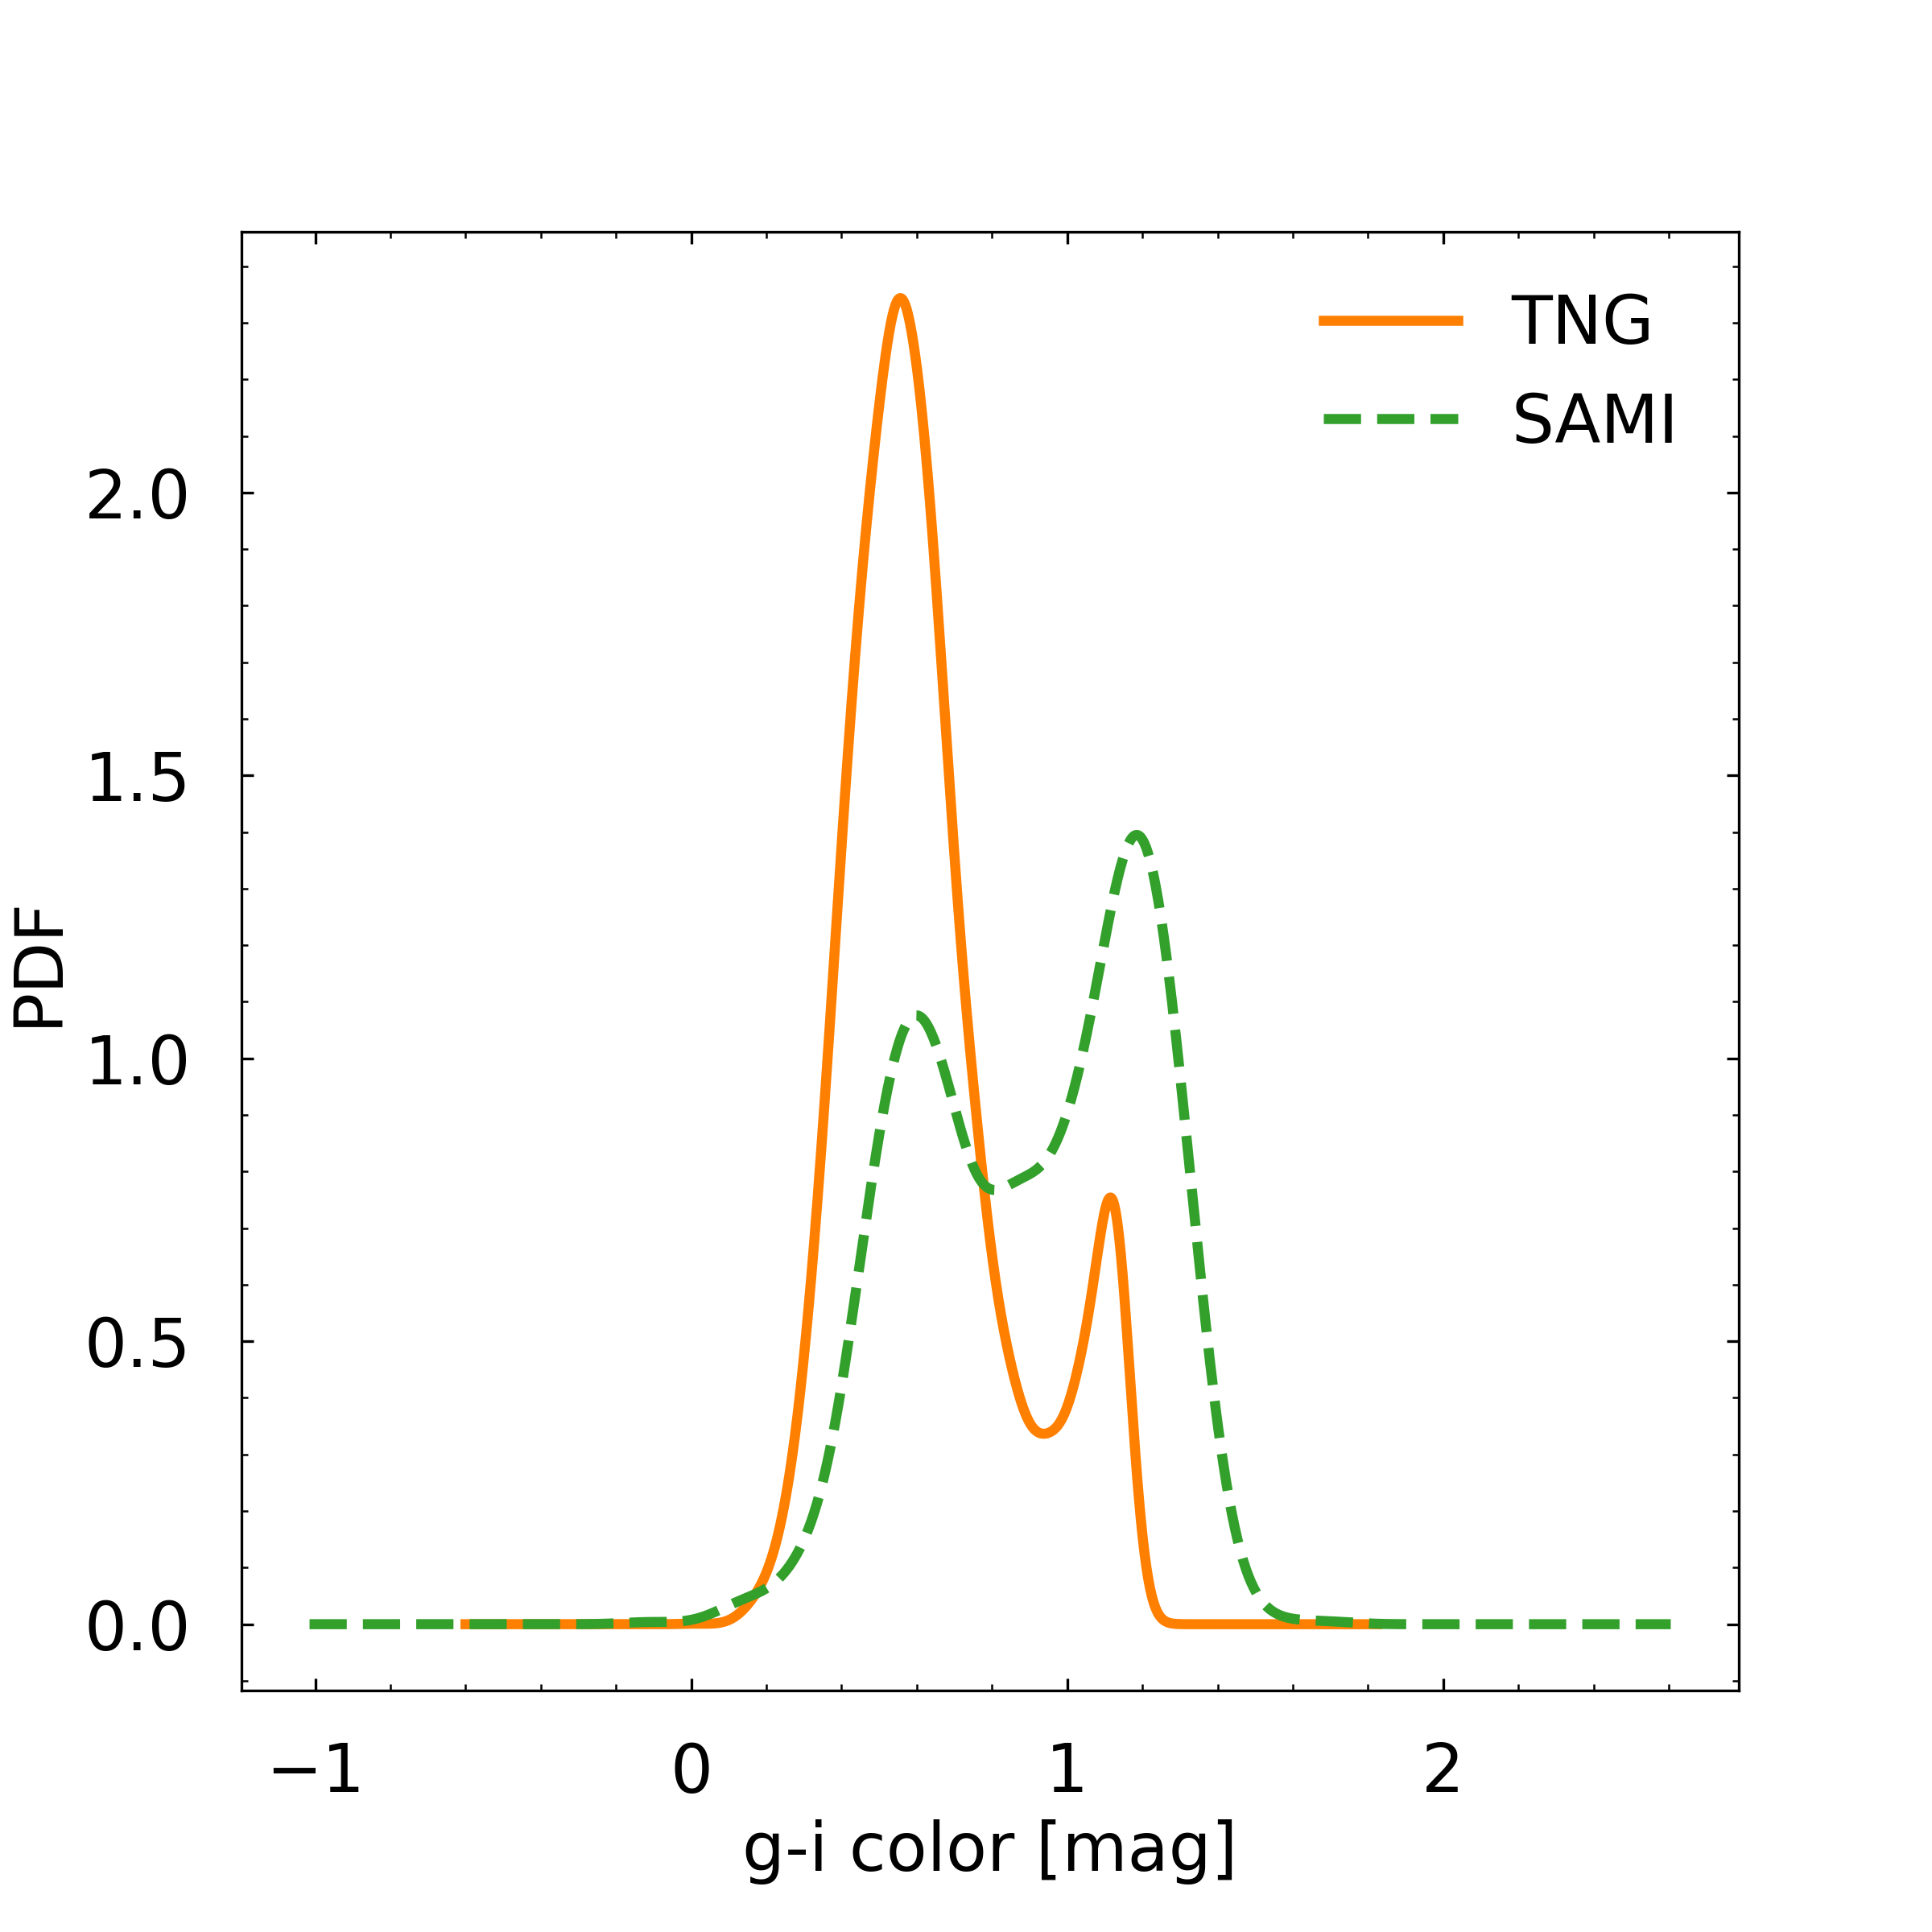
\includegraphics[width=0.9\textwidth]{images/results_pdf_g_i_band.png}
    \caption{}
    \label{pdf_color_res2}
\end{figure}

\subsection{SMBH relations}
In Figure \ref{bh_res} the SMBH-mass and velocity dispersion for TNG100 is shown, along with the best fit functions from \cite{Ferrarese2000} and \cite{Tundo2007}.

\begin{figure}
    \centering
    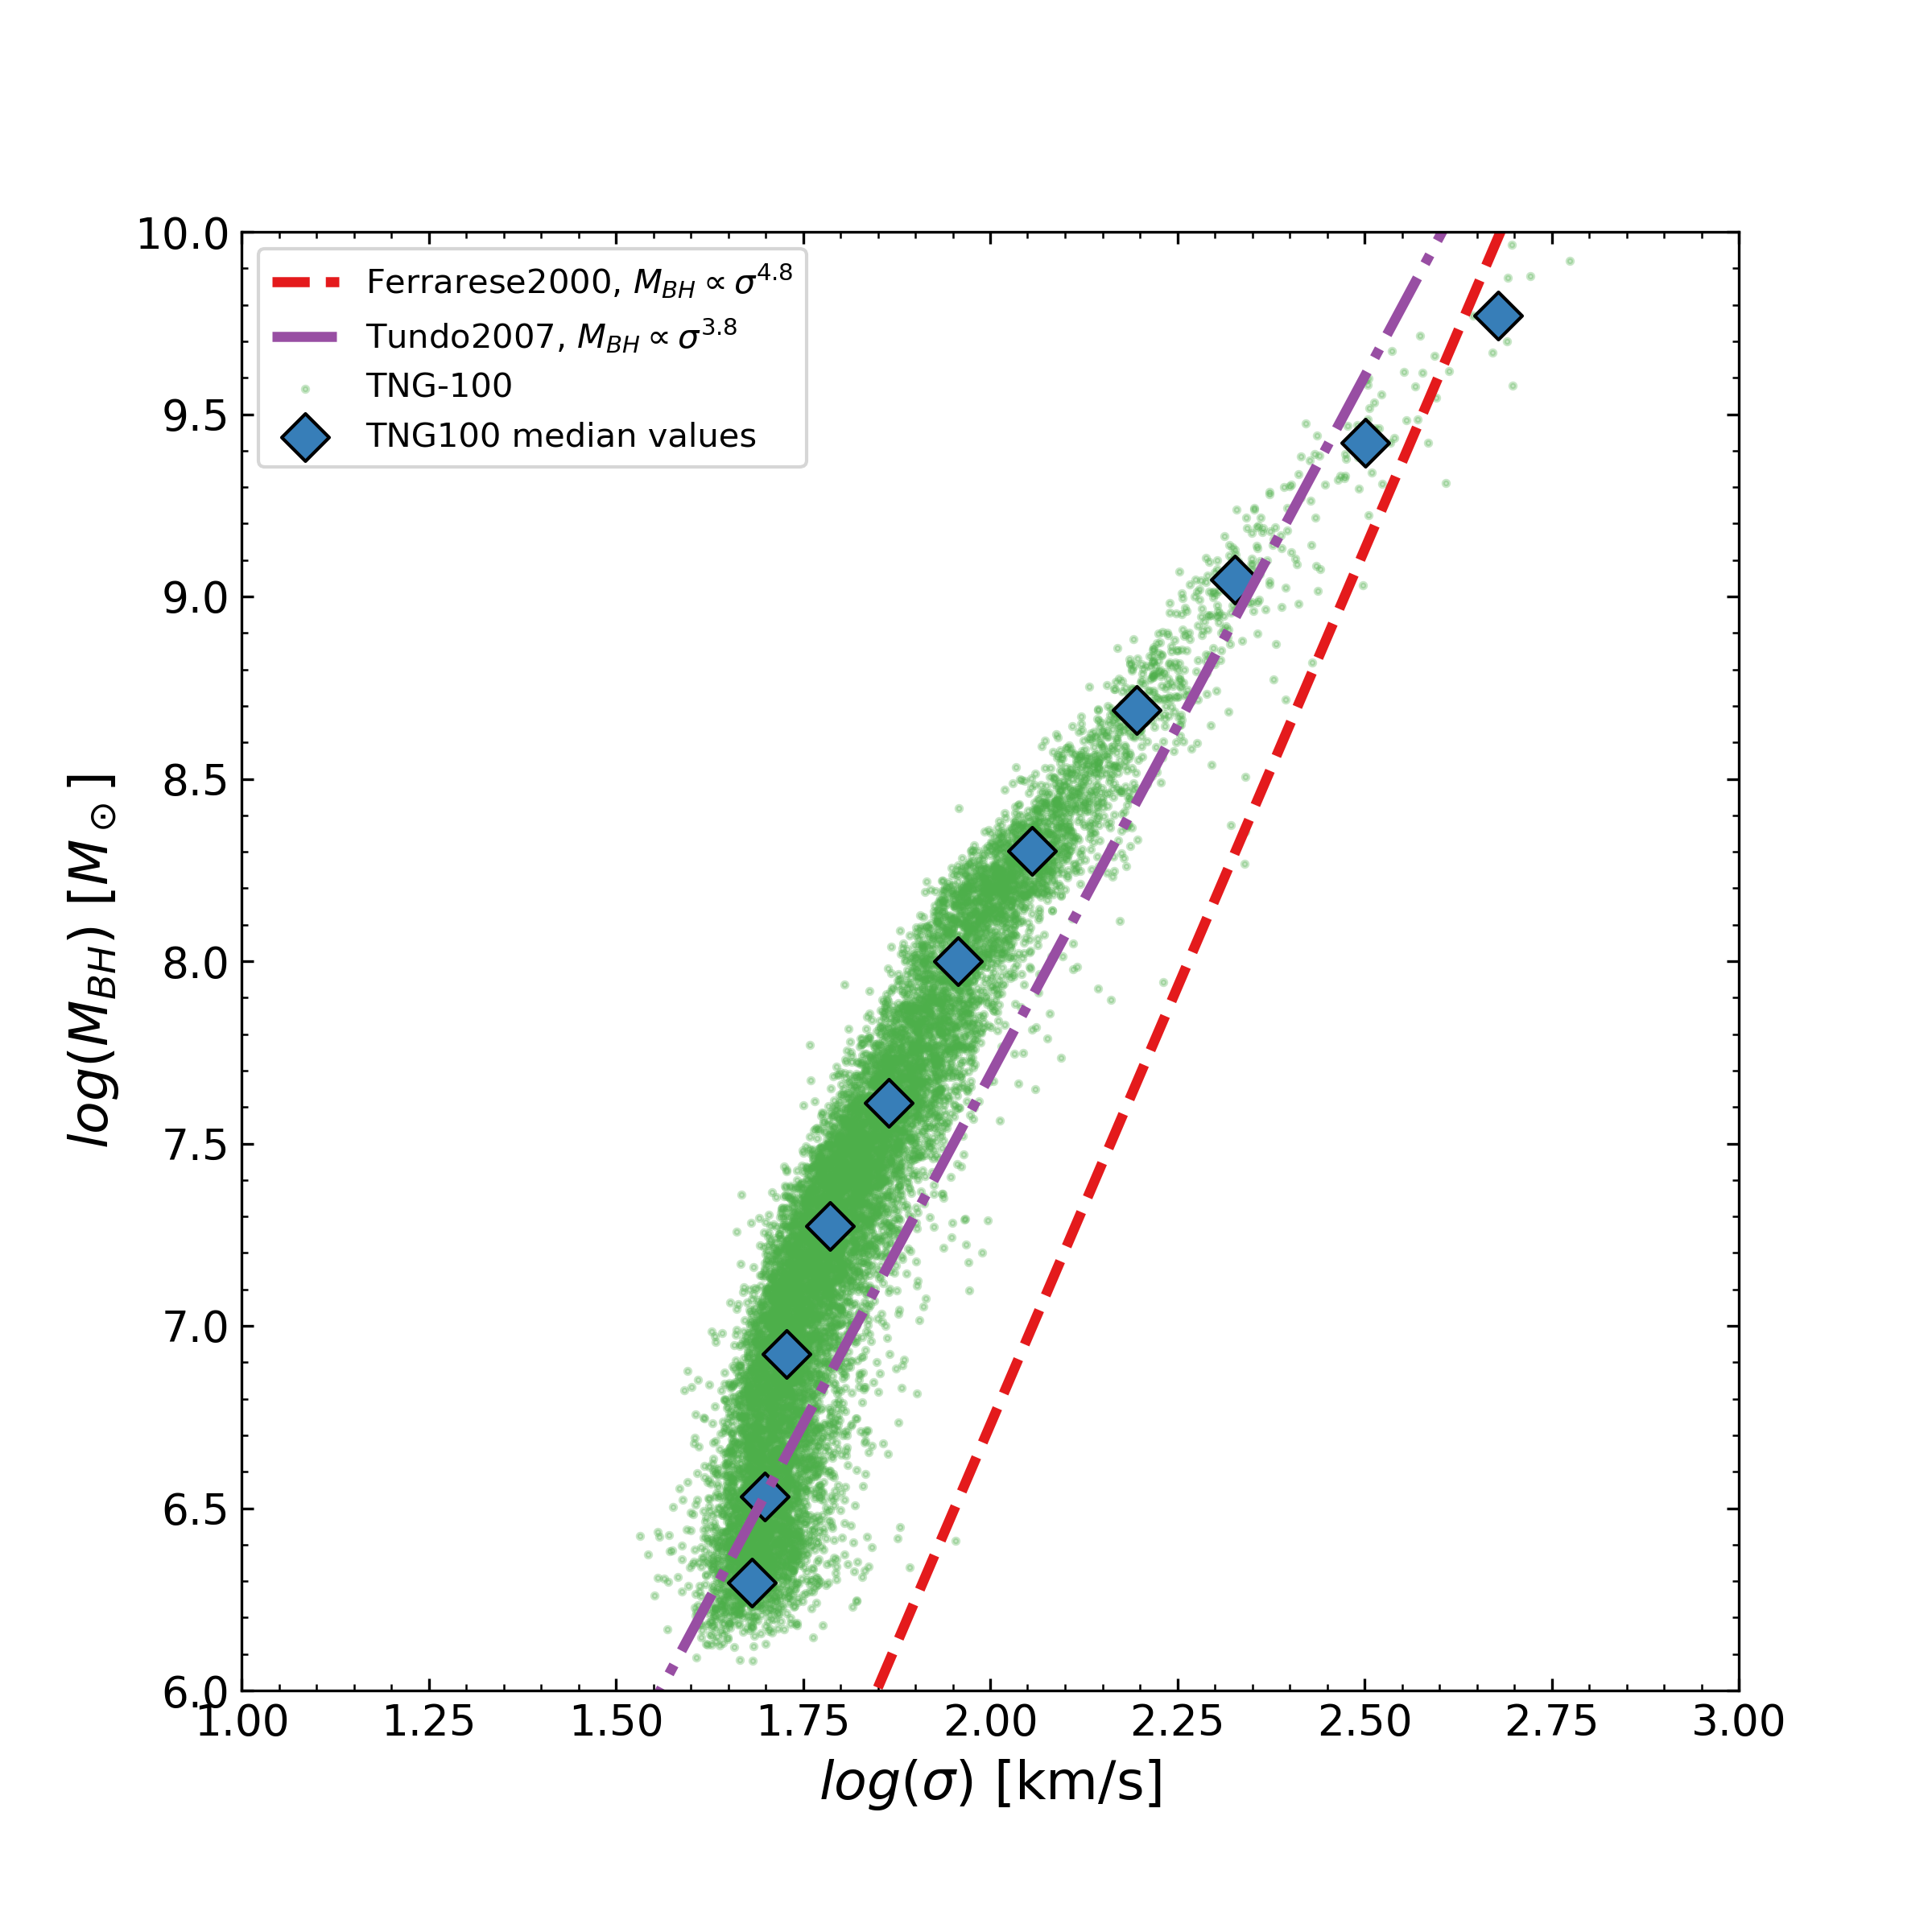
\includegraphics[width=0.9\textwidth]{images/results_mass_BH_sigma.png}
    \caption{}
    \label{bh_res}
\end{figure}